\documentclass[letterpaper,final,12pt,reqno]{amsart}

\usepackage[total={6.3in,9.2in},top=1.1in,left=1.1in]{geometry}

\usepackage{times,bm,bbm,empheq,fancyvrb,graphicx}
\usepackage[dvipsnames]{xcolor}
\usepackage{tikz}

% hyperref should be the last package we load
\usepackage[pdftex,
colorlinks=true,
plainpages=false, % only if colorlinks=true
linkcolor=blue,   % ...
citecolor=Red,    % ...
urlcolor=black    % ...
]{hyperref}

\renewcommand{\baselinestretch}{1.05}

\newtheorem{lemma}{Lemma}

\newcommand{\Matlab}{\textsc{Matlab}\xspace}
\newcommand{\eps}{\epsilon}
\newcommand{\RR}{\mathbb{R}}

\newcommand{\grad}{\nabla}
\newcommand{\Div}{\nabla\cdot}
\newcommand{\trace}{\operatorname{tr}}

\newcommand{\hbn}{\hat{\mathbf{n}}}

\newcommand{\bg}{\mathbf{g}}
\newcommand{\bn}{\mathbf{n}}
\newcommand{\bu}{\mathbf{u}}
\newcommand{\bv}{\mathbf{v}}
\newcommand{\bx}{\mathbf{x}}

\newcommand{\bV}{\mathbf{V}}
\newcommand{\bX}{\mathbf{X}}

\newcommand{\bxi}{\bm{\xi}}

\newcommand{\bzero}{\bm{0}}

\newcommand{\rhoi}{\rho_{\text{i}}}

\newcommand{\cref}{c_{\text{ref}}}
\newcommand{\Href}{H_{\text{ref}}}
\newcommand{\num}{\nu_{\text{m}}}
\newcommand{\rhom}{\rho_{\text{m}}}


\begin{document}
\title[Evolving-geometry glacier and ice sheet simulations using Stokes dynamics]{Evolving-geometry glacier and ice sheet simulations \\ using Stokes dynamics}

\author{Ed Bueler}

% Co-author thoughts:
%   * L.~Mitchell because of \texttt{SemiCoarsened...()} etc.~ code (actual)
%   * C.~Khrulev because of implementation and analysis help (prospect)
%   * R.~Sayag because of validation experiment (prospect)
%   * M.~Knepley because of performance help and analysis (prospect)
%   * D.~Shapero because of firedrake help (actual) and implementation or application (prospect)

\maketitle

\thispagestyle{empty}
\bigskip

\section{Introduction} \label{sec:intro}

The most important questions in glaciology concern how the climate around a glacier determines its geometry, both through mass balance and stresses along the ice surface and through internal flow dynamics.  In particular, relationships between surface mass inputs and the geometry of the ice mass are important because they affect sea level, deformations of the Earth's crust, and fresh water supplies, among other concerns.  In this context, evolving-geometry simulations are widely used by scientists to understand the size and extent of glaciers and ice sheets.  A variety of methodologies for such numerical simulations are seen in practice, with most of the well-established schemes involving shallowness approximations of the continuum equations \cite[for example]{Hoffmanetal2018,Lipscombetal2019,Winkelmannetal2011}.  Furthermore, most methods use explicit or semi-implicit time-stepping \cite{HindmarshPayne1996,Hoffmanetal2018,Lipscombetal2019,Winkelmannetal2011}, with small stability-imposed time steps at high spatial resolution, though fully-implicit exceptions exist \cite{Brinkerhoffetal2017,Bueler2016}.  The performance properties of current numerical models therefore limit either the physical modeling authenticity (due to shallowness and other approximations) or the spatial resolution (due to time-stepping and solver performance limitations).  In particular, the quality of ensemble simulations, regarding both the number of ensemble members and the quality of the individual simulations, is directly limited by numerical model performance.

This paper\footnote{version: \today.} addresses an important, but also restricted, class of numerical glacier and ice sheet models which are based on conservation of momentum and mass and which avoid shallowness assumptions.  For conservation of momentum we use the standard shear-thinning (Glen) power-law Stokes model.  Noting that ``mass conservation'' properly refers both to fluid incompressibility and to conservation at the ice surface, we simultaneously solve the stress balance and zero divergence equations for bulk ice and the surface kinematical equation (or kinematic boundary condition \cite{GreveBlatter2009}) with the surface mass balance is an input.  We model three-dimensional (3D) grounded glaciers and ice sheets for which there is a well-defined ice thickness; overhanging ice is not modeled.  Note that the ice thickness is defined at all map-plane points but it is zero in those locations where the (coupled and solved) surface balance and ice flow do not determine the presence of glacier ice.  The solution process also determines the location of the free boundary at the ice margin \cite{SchoofHewitt2013} (Figure \ref{fig:context}).

\begin{figure}[ht]
\begin{center}
\includegraphics[width=0.7\textwidth]{figs/context.pdf}
\end{center}
\caption{We consider 3D models of grounded glaciers and ice sheets which are based on Glen-Stokes ice flow, an evolving free surface, and a free boundary.}
\label{fig:context}
\end{figure}

We do not, however, consider the conservation of energy, and neither thermomechanical coupling nor basal melt are included in our model.  A further restriction is that our ice sticks to the bed (no slip), and we do not consider floating ice.  Finally we only consider cases where the bed elevations are relatively-smooth.  These restrictions are all removable by well-known modeling mechanisms \cite[for example]{Aschwandenetal2012,Winkelmannetal2011}, but how these components affect the performance or fully-coupled implicit time-stepping models like the one here is a topic for further research.

To discretize the continuum equations we apply the finite element (FE) method \cite{Elmanetal2014} by using the Firedrake library \cite{Rathgeberetal2016} in Python.\footnote{These Python programs are open-source at \href{https://github.com/bueler/stokes-implicit}{\texttt{github.com/bueler/stokes-implicit}}.  FIXME: MAKE REPO PUBLIC.}  We use meshes which are unstructured in the map-plane but which are extruded \cite{Bercea2016,Gibsonetal2019,McRaeetal2016} in the vertical direction.  As discussed below, mixed elements for velocity, pressure, and vertical ice strain are used, with stable and aspect-ratio robust choices for the velocity-pressure (i.e.~Stokes) block \cite{Elmanetal2014}.  Solutions of the resulting nonlinear discrete equations apply multigrid-preconditioned Newton-Krylov methods \cite{Bueler2021} via PETSc \cite{Balayetal2020}, with semicoarsening in the vertical direction \cite{Tuminaroetal2016}, and all computations are parallelized.

FIXME compare literature of existing solvers:
\begin{itemize}
\item  nonevolving surface Stokes \cite{IsaacStadlerGhattas2015,Lengetal2013,Lengetal2014a,Zwingeretal2007} (CHECK)
\item  explicitly evolving surface \cite{Gudmundsson1999,HelanowAhlkrona2018,Jouvetetal2008,Larouretal2012,
Lengetal2014b,Lengetal2012,LeysingerGudmundsson2004,PralongFunk2004,Seddiketal2012} (CHECK)
\item significant hydrostatic/B-P \cite{BrownSmithAhmadia2013,Tuminaroetal2016}
\end{itemize}

One model performance metric introduced here is a natural one for glacier modeling.  Namely, we measure the run time of our coupled Glen-Stokes simulations relative to the well-understood computation of ice velocity in the shallow ice approximation (SIA) \cite{Fowler1997} on the same mesh.  That is, we define a glacier model ``work unit'' as the time needed for a diagnostic computation of the SIA horizontal velocity solution.

The primary purpose of this paper is to understand the performance characteristics of numerical simulations using fully-implicit time-stepping with evolving-surface Glen-Stokes models.  At each time step the stress balance, incompressibility, and surface kinematical equations are solved simultaneously to within a tolerance on the coupled residual.  Time steps of order one year are targeted but we identify geometry error metrics which are used to limit and adjust time steps.  To evaluate our approach we validate the model based on results of laboratory experiments, we compare the performance of the model with shallow models, we demonstrate solver optimality and scalability, and we show a solution for the Greenland ice sheet.  At the end we identify spatial resolutions at which the performance of our non-shallow model will actually exceed that of explicit time-stepping SIA models.


\section{Equations for ice flow in glaciers} \label{sec:strongform}

The standard model for the flow of glaciers uses Stokes equations based upon Glen's shear-thinning flow law for ice \cite{GreveBlatter2009,JouvetRappaz2011,SchoofHewitt2013}.  We will apply this model on time-dependent $d=2$ or $d=3$ dimensional domains using time $t>0$ and spatial variables $\bx=(x,y,z)$, with $z$ vertical.  We present the equations assuming $d=3$, but note that coordinates are denoted $(x,z)$ in 2D.  The evolving domain $\Omega^t \subset \RR^d$ will have a piecewise smooth boundary, so that we may apply the boundary conditions, but it is otherwise general.

Allowing any Glen exponent $n\ge 1$, the strong-form model equations for bulk ice are:
\begin{align}
- \nabla \cdot \tau + \nabla p &= \rhoi \bg &&\text{\emph{stress balance}} \label{forcebalance} \\
\nabla \cdot \bu &= 0 &&\text{\emph{incompressibility}} \label{incompressible} \\
\tau &= B_n |D\bu|^{(1/n) - 1} D\bu  &&\text{\emph{flow law}} \label{viscflowlaw}
\end{align}
The solution fields are velocity $\bu$, pressure $p$, and deviatoric stress tensor $\tau$.  For simplicity we take the ice density $\rhoi$ and the acceleration of gravity $\bg=\left<0,0,-g\right>$, with $g>0$, to be constant.

Regarding tensors and their notation, the full (Cauchy) stress tensor $\sigma$ \cite{GreveBlatter2009} decomposes into the deviatoric part $\tau$ minus the pressure, i.e.~$\sigma = \tau - p\,I$, so equation \eqref{forcebalance} simply says $-\Div \sigma = \rhoi \bg$.  The strain rate tensor $D\bu$ is the symmetric part of $\grad \bu$, i.e.~$(D\bu)_{ij} = \frac{1}{2} \left(\grad\bu + \grad\bu^\top\right)$.  Because $D\bu$ is symmetric, and because it has trace zero by equation \eqref{incompressible}, i.e.~$\trace(D\bu)=\nabla \cdot \bu = 0$, from equation \eqref{viscflowlaw} it follows that $\tau$ is also symmetric with trace zero.  The tensor norm in \eqref{viscflowlaw} satisfies $|D\bu|^2 = \frac{1}{2} \trace\left((D\bu)^2\right) = \frac{1}{2} (D\bu)_{ij} (D\bu)_{ij}$.  Note $B_n$ is the $n$-dependent ice hardness in units $\text{Pa}\,\text{s}^{1/n}$, sometimes written $B_n = (A_n)^{-1/n}$ in terms of the softness $A_n$.

For the linear Stokes equations \cite{Elmanetal2014}, i.e.~the $n=1$ case, one would traditionally write the flow law \eqref{viscflowlaw} as $\tau = 2\nu D\bu$, and in that case the viscosity would be $\nu = (1/2) B_1$.  For powers $n>1$, namely shear-thinning ice, one defines an ``effective viscosity'' in equation \eqref{viscflowlaw} which involves a negative power of the strain rate norm $|D\bu|$.  This effective viscosity would be singular in the limit of small strain rates, and so, motivated by the expected finite viscosity of glacier ice \cite{GreveBlatter2009}, and noting that the equations using such a regularization are well-posed \cite{JouvetRappaz2011}, we define the regularized effective viscosity
\begin{equation}
\nu_\eps(|D\bu|) = \frac{1}{2} B_n \left(|D\bu|^2 + \eps\, D_0^2\right)^{(r-2)/2} \label{regeffvisc}
\end{equation}
where $\eps = 10^{-4}$ and $r=(1/n)+1$.  The constant $D_0$ defines a strain-rate scale for glacier flow; the value $D_0 = 2 \,\text{a}^{-1}$ used here corresponds to a velocity difference of 1000 meters per year in a distance of 500 meters.

Using \eqref{viscflowlaw} as modified by \eqref{regeffvisc}, we eliminate $\tau$ from equation \eqref{forcebalance} and rewrite the system in terms of velocity and pressure derivatives only:
\begin{align}
- \nabla \cdot \left(2 \nu_\eps(|D\bu|)\, D\bu\right) + \nabla p &= \rhoi \mathbf{g} \label{stokes} \\
\Div \bu &= 0 \label{incompagain}
\end{align}
This system is our Glen-Stokes model for bulk ice motion.  The solution is a velocity-pressure pair $(\bu,p)$, from which one may derive strain rates $D\bu$ and stresses $\tau$ and/or $\sigma = \tau - p\,I$.

Glacier-suitable dynamic boundary conditions will be used, with an emphasis on isolated, grounded glaciers and ice sheets.  In such cases the ice flow extends in the horizontal direction until a free boundary at the glacier margin is reached.  (Note that glacier margins may occur as fracture-generated cliffs, but such non-fluid processes are not modeled here.)  As noted in the Introduction, we assume that the ice thickness is well-defined and thus that the top and bottom boundaries of $\Omega^t$ can, at each time, be identified.  On the top surface we set a condition of zero applied stress,
\begin{align}
\left(2 \nu_\eps(|D\bu|) D\bu - pI\right) \bn &= \bzero  &&\text{\emph{top}: } \overline{\partial} \Omega^t \label{topbc} \\
\intertext{where $\bn$ is normal to the surface.  On the base we require no slip:}
\bu &= \bzero  &&\text{\emph{base}: } \underline{\partial} \Omega^t \label{basebc}
\end{align}

Optionally, to allow simulation of a certain laboratory experiment \cite{SayagWorster2013} (below), we also allow inflow.  Here a prescribed velocity is applied, $\bu = \bu_{\text{in}}$ on an inflow boundary $\partial_{\text{in}} \Omega^t$, subject to $\bu_{\text{in}}\cdot \bn \le 0$ where $\bn$ is an outward normal.

Assuming the well-posedness of the above model \eqref{stokes}--\eqref{basebc}, as proven by \cite{JouvetRappaz2011}, if the ice geometry $\Omega^t$ is known then the solution is a unique pair $(\bu,p)$.  Note that the slowness of the fluid, i.e.~zero Reynolds number, implies that for a fixed domain $\Omega^t$ the boundary stresses and body forces determine velocity and pressure fields without any ``memory'' of prior states or influence from inertia, as would occur in the Navier-Stokes equations \cite{Fowler1997}.


\section{Ice geometry evolution} \label{sec:stronggeometry}

The above equations do not describe how a glacier changes shape or extent.  This process, which is coupled to the flow velocity but not fully determined by it, is described by an additional equation which states conservation of mass on the top boundary $\overline{\partial} \Omega^t$.  To present this equation we first assume a larger map-plane computational domain $R\subset \RR^{d-1}=\RR^2$ on which the surface mass balance and bedrock elevation data of the problem are defined; see Figure \ref{fig:domainnotation}.  The ice-covered area is then a subset of the interior of $R$.  In fact, we will consider only isolated glaciers and ice sheets, so ice must not be present on, nor flow across, the boundary of $R$.

Let $z=b(x,y)$ be the bedrock elevation, assumed continuously-differentiable and time-independent for simplicity, and $z=h(t,x,y)$ the ice surface elevation; note that both functions are defined for all $(x,y)\in R$.  The function $h$ is part of the solution while $b$ is input data.  The following form for the time-dependent, open ice domain is now assumed:
\begin{equation}
\Omega^t = \left\{\bx\,\big|\,(x,y)\in R \,\text{ and }\, b(x,y) < z < h(t,x,y)\right\}.  \label{Omegat}
\end{equation}
Note that an admissibility requirement for $h$, as a part of the model solution, is that at each $t>0$ and $(x,y)\in R$ we have $h(t,x,y) \ge b(x,y)$.  On the other hand, at any given map-plane location $(x,y)$ the ice may be present (strict inequality) or absent (equality) in an evolving, time-dependent manner.  Also, as shown in Figure \ref{fig:domainnotation}, the ice-covered map-plane domain, the vertical projection of $\Omega^t$, will be denoted $\pi \Omega^t$.

\begin{figure}[ht]
\begin{center}
\includegraphics[width=0.7\textwidth]{figs/domainnotation.pdf}
\end{center}
\caption{Notation: The evolving ice domain $\Omega^t$ has projection $\pi \Omega^t$.  Surface mass balance $a$ and bedrock elevation $b$ are defined on all of $R$.}
\label{fig:domainnotation}
\end{figure}

In agreement with almost all ice sheet and glacier modeling literature, \eqref{Omegat} states that both the upper and lower surfaces of the ice mass are described by a well-defined functions of map-plane location.  The domain $\Omega^t$ is thus a layer \cite{Bueler2020}, and not general.  Furthermore we assume a disjoint boundary decomposition $\partial \Omega^t = \overline{\partial} \Omega^t \cup \underline{\partial} \Omega^t$, except for a set of measure zero along the margin.\footnote{An exception to this assertion is for an inflow: $\partial_{\text{in}} \Omega^t \ne \emptyset$.}  Looking ahead, this layer assumption is compatible with our FE method based on a vertically-extruded, unstructured mesh in the map plane.

Let $a_\perp(t,x,y,z)$ be the modeled vertical climatic surface mass balance, in (ice-equivalent) units $\text{m}\,\text{s}^{-1}$.  This scalar field must be defined for all locations above the bedrock elevation, i.e.~$(x,y,z) \in R\times[b(x,y),\infty)$.  Denoting the velocity components as $\bu=\left<u,v,w\right>$, the surface kinematical equation \cite{GreveBlatter2009} then applies on the top of the ice, namely $\frac{\partial h}{\partial t} = a - u \frac{\partial h}{\partial x} - v \frac{\partial h}{\partial y} + w$ or, stated using vector notation,
\begin{equation}
\frac{\partial h}{\partial t} = a + \bu \cdot \bn \quad \text{ on } \overline{\partial}\Omega^t, \label{surfacekinematical}
\end{equation}
where $\bn = \left<-\frac{\partial h}{\partial x},-\frac{\partial h}{\partial y},1\right>$ points upward and is normal to the ice surface.  The surface mass balance $a$ in \eqref{surfacekinematical} is the trace \cite{Evans2010} of the mass balance along the ice surface, i.e.~$a = a_{\perp}(t,x,y,h(t,x,y))$, and similarly for the velocity $\bu = \bu(t,x,y,h(t,x,y))$.  Note that, because $\bn$ points along $-\grad h$, equation \eqref{surfacekinematical} is often regarded as similar to an advection of $h$ or of the ice thickness.  However, ice also tends to flow downhill---vaguely speaking $\bu \sim -\grad h$---so the equation is diffusive at large scale.

Modeled melting or freeze-on at the ice base would add a basal kinematic equation \cite[for example]{Aschwandenetal2012}, but for simplicity this is not considered here.

Equation \eqref{surfacekinematical} applies on the ice surface, that is, where ice is present.  However, the equation should be understood as the following statements which hold on the entire computational domain $R$ \cite{SchoofHewitt2013}:
\begin{align}
h-b &\ge 0, \label{strongadmissibility} \\
\frac{\partial h}{\partial t} - a - \bu \cdot \bn &\ge 0, \label{stronginequality} \\
(h-b) \left(\frac{\partial h}{\partial t} - a - \bu \cdot \bn\right) &= 0. \label{strongcomplementarity}
\end{align}
These statements, which form a nonlinear complementarity problem (NCP) \cite{Bueler2016,Bueler2020}, avoid referring to glacier extent, which we must regard as part of the solution.  Equation \eqref{strongcomplementarity}, the complementarity principle, says that either there is no ice at the location ($h=b$) or ice is present and equation \eqref{surfacekinematical} applies.  At ice-free locations, where $h=b$, $\partial h/\partial t=0$, and $\bu=\bzero$, \eqref{stronginequality} says that $a \le 0$, that is, the surface mass balance is not positive.  (Otherwise, assuming continuity for $a$, there would have been ice.)  Physically-speaking, at such locations snow melt and runoff exceed solid precipitation, and ice has not been able to flow there either.

The NCP \eqref{strongadmissibility}--\eqref{strongcomplementarity} can be regarded as having only the surface elevation $h$ as the unknown or state vector.  In particular, where $\bu$ appears in the NCP, being a solution $(\bu,p)$ of the Stokes problem \eqref{stokes}--\eqref{basebc}, it is the image of a nonlinear and nonlocal map from ice geometry to the surface value (trace) of the solution velocity $\bu$.  That is, the surface velocity $\bu$ in the surface kinematical equation, whether stated as the classic equation \eqref{surfacekinematical} or through the NCP, can be written as ``$\bu(h,b)$'' if desired.  (In the current paper, bed elevation $b$ is fixed data.)

Informally, the surface kinematical equation describes how the ice surface elevation is updated: the climatically added or removed ice $a\,\Delta t$, plus the component of the ice motion in direction $\bn$, determines the vertical displacement of the surface.  Numerical glacier models therefore often evolve the time-dependent surface $z=h$ by explicit steps, i.e.~$\Delta h \approx \left(a + \bu\cdot \bn\right) \Delta t$ in the simplest forward-Euler case, based upon the current values of $a$, $\bu$, and $\bn$ (i.e.~$\grad h$).  However, we will be solving \eqref{surfacekinematical}, more precisely \eqref{strongadmissibility}--\eqref{strongcomplementarity}, implicitly and coupled with the Glen-Stokes system \eqref{stokes}--\eqref{basebc}.  The new ice surface will be compatible with the flow model when the solver has converged.

Note that the mass balance $a_{\perp}(t,x,y,z)$ is computed using a separate model for the dynamical state of the atmosphere, one which computes snow precipitation, (atmospheric) energy-driven melt at snow/ice surfaces, and liquid water runoff.  How this is done is well beyond our scope, but it is important in moving-margin glacier simulations that $a$ have a well-defined value both at the current ice surface and elsewhere, or at least nearby.  This is because a simulated glacier can only move into new areas, retreat from ice-covered areas, and undergo changes of surface elevation, if the source term at the new (and intermediate) locations is well-defined.  This issue can be ignored for explicit time-steps, but not here.

Appendix A summarizes a simplified model of our main coupled problem, namely the shallow ice approximation (SIA), but we will only need it as a source of initial conditions and in performance comparisons.


\section{Implicit time-stepping and the domain update} \label{sec:implicitstep}

Our main purpose is to demonstrate an implicit scheme to simultaneously solve the Glen-Stokes problem \eqref{stokes}--\eqref{basebc} and the surface kinematical equation \eqref{surfacekinematical}.  The only time derivative in this coupled problem appears in equation \eqref{surfacekinematical}.  Because the remaining equations and boundary conditions lack time derivatives, but they apply at all times, the coupled problem should be understood as an infinite-dimensional differential algebraic equation (DAE) problem \cite{AscherPetzold1998}.  In this section, using a discrete-time and continuous-space formulation, we state our scheme for solving this problem.  A new feature is that at each time step we compute a vertical-only displacement field which captures the effect of the surface kinematical equation along the boundary but which is defined everywhere within the same (reference) domain as the velocity and pressure.  The coupled solution, once found, includes this vertical displacement which then determines the new 3D domain of ice at the end of the time step.

We discretize the coupled problem in time using the first-order backward Euler method.  Higher-order implicit schemes exist, including stiff-decay backward-differentiation schemes \cite{AscherPetzold1998,Bueler2021} suitable for DAE problems.  However, because the coupled solution is also subject to inequality constraints \eqref{strongadmissibility}--\eqref{strongcomplementarity}, this free-boundary problem has the character of a time-dependent NCP, as in section \ref{sec:stronggeometry}, or a variational inequality \cite{Calvoetal2002} problem.  The numerical errors associated to determining the free boundary are unavoidably of low order in time and space \cite{Bueler2020} and thus they tend to dominate over time-stepping errors made in well-behaved locations.  Effective application of higher-order time-stepping is thus a topic for future research.

The fundamental issue faced by implicit time-stepping schemes for glaciers is that the map-plane (2D) region covered by ice changes during the time step.  Either in terms of the 3D continuum domain of the coupled PDE problem, or in terms of the 3D mesh used for numerical simulations, one can only solve for ice velocity and pressure in locations where ice or mesh, respectively, exists.  Concretely, supposing $t_{n-1}$ and $t_n$ are consecutive times with step $\Delta t = t_n - t_{n-1} > 0$, the possibility of glacier advance and retreat during an implicit step requires the PDE domain to cover the current ice (time $t_{n-1}$), and yet we must also extend the domain to locations where ice might be present once we have solved the equations for the new time ($t_n$).

\begin{figure}[ht]
\begin{center}
\includegraphics[width=0.65\textwidth]{figs/currenttime.pdf}
\vspace{-6mm}

\includegraphics[width=0.65\textwidth]{figs/referencedomain.pdf}
\vspace{-1mm}

\includegraphics[width=0.65\textwidth]{figs/nexttime.pdf}
\end{center}
\caption{The current ice domain $\Omega^{n-1}$ is used to construct a reference domain $\Lambda$.  The coupled solution on $\Lambda$ generates a map from $\Lambda$ to the new domain $\Omega^n$.}
\label{fig:domainupdate}
\end{figure}

Our scheme uses the current ice geometry to construct a reference domain on which the new velocity, pressure, and vertical displacement are found as the coupled problem is solved.  The detailed construction of the reference domain, given next, is not as important as the main idea that the coupled PDE solution must occur on a domain supporting the new ice geometry, while also being defined where ice currently exists, because the current ice surface elevation is a term in the discrete-time equations (below).  The icy domain must be allowed to change, including either elimination or creation of ice in a given map-plane location, so changes in the map-plane topology, as a glacier disconnects for example, must be allowed.

For this construction we need a reference glacier thickness $\Href>0$, a value such that grounded ice of uniform thickness $\Href$ flows slowly over the bedrock topography, and which is small compared to observed glacier thicknesses.  For example, the range $50 \le \Href \le 500$ m, for small mountain glaciers up to large, cold, and low-angle ice sheets, is appropriate.  Recall that the velocity of Glen $n=3$ ice in a slab-on-slope geometry \cite{GreveBlatter2009} goes as the $4$th power of the ice thickness, and thus $50$ m ice flows $10^4$ times slower than $500$ m ice.

Suppose $h^{n-1}(x,y) \approx h(t_{n-1},x,y)$ is our current surface elevation.  Denote the corresponding ice domain by $\Omega^{n-1}=\{\bx\,\big|\,(x,y)\in R, b(x,y)<z<h^{n-1}(x,y)\} \subset \RR^3$; see \eqref{Omegat} and the top of Figure \ref{fig:domainupdate}.  The reference domain will have thickness which is everywhere at least $\Href$, so for $(x,y) \in R$ let
\begin{equation}
\lambda(x,y) = b(x,y) + \max\{\Href,h^{n-1}(x,y)-b(x,y)\}. \label{definelambda}
\end{equation}
Define the reference domain to have surface $z=\lambda(x,y)$:
\begin{equation}
\Lambda = \left\{(\xi,\eta,\zeta)\,\big|\,(\xi,\eta)\in R, \, b(\xi,\eta) < \zeta < \lambda(\xi,\eta)\right\};  \label{Lambda}
\end{equation}
see Figure \ref{fig:domainupdate}.  Observe that $\Omega^{n-1} \subset \Lambda$ and $h^{n-1} \le \lambda$, and that $\Lambda$ and $\lambda$ are fully determined by data which is known at the start of the time step.

From now on $\bxi=(\xi,\eta,\zeta)$ will denote coordinates on $\Lambda \subset \RR^3$.  We will compute the updated domain $\Omega^n \subset \RR^3$ via a change of coordinates, a map $\bxi \mapsto \bx$:
\begin{equation}
\bx(\bxi) = \bxi + (0,0,c(\bxi)). \label{changecoords}
\end{equation}
This map is based on a new scalar function $c(\bxi)$ which is defined on $\Lambda$ and satisfies certain properties.  One of these is that
\begin{equation}
c(\xi,\eta,b(\xi,\eta))=0, \label{mapbasetobase}
\end{equation}
thus the map preserves the elevation of the bedrock.  Note that the horizontal coordinate is unchanged, but the $z$-coordinate $z(\xi,\eta,\zeta)=\zeta+c(\xi,\eta,\zeta)$ is nontrivial.

The domain $\Omega^n$ is defined to be the interior of the image of $\Lambda$ under map \eqref{changecoords}:
\begin{equation}
\Omega^n = \{\bx(\bxi) \,\big|\, \bxi \in \Lambda\}^\circ. \label{updateddomain}
\end{equation}
Determining $c(\bxi)$ on $\Lambda$ will therefore determine the new ice domain $\Omega^n$.  Since $c(\bxi)$ will solve an elliptic PDE (below), the map is smooth from $\Lambda$ to $\Omega^n$, but it is degenerate.  It is not a diffeomorphism because its inverse is not generally smooth or even well-defined.  In particular, applying the topological interior in \eqref{updateddomain} is important because the map will take ice free locations in $\Lambda$ to locations which have zero height and are outside of $\Omega^n$.

We now assume that map \eqref{changecoords} is monotonic in each column where ice is present in the solution, that is, that for each fixed $(\xi,\eta)\in R$ the map $f(\cdot) = z(\xi,\eta,\cdot)$ takes the interval $I=(b(\xi,\eta),\lambda(\xi,\eta))$ monotonically to a new interval in a nondecreasing manner.  We include the possibility that $I$ is mapped to a single point.  Consider the computed surface elevation $h(\xi,\eta)\approx h(t_n,\xi,\eta)$, which includes the upper boundary of $\Omega^n$ but which is defined on all of $R$.  It follows by maximizing\footnote{I.e.~taking the supremum of $f$.} $f$ in each column that $h(\xi,\eta)$ satisfies
\begin{equation}
h(\xi,\eta) = \lambda(\xi,\eta) + c(\xi,\eta,\lambda(\xi,\eta)) \label{maptoptotop}
\end{equation}
at all locations $(\xi,\eta)\in R$.  That is, the top of the reference domain is sent to the top of the new ice domain.  Furthermore, because the map is differentiable, and because of \eqref{mapbasetobase} and \eqref{maptoptotop}, the mean value theorem implies
\begin{equation}
1 + \frac{\partial c}{\partial \zeta}(\bxi) = \frac{\partial z}{\partial \zeta}(\bxi) \ge 0. \label{mapmonotonic}
\end{equation}
Finally, in locations which are computed to be ice free we have
\begin{equation}
h(\xi,\eta)=b(\xi,\eta) \quad \implies \quad b(\xi,\eta) = \zeta + c(\xi,\eta,\zeta) \text{ for all } \zeta \in I, \label{mapcrushes}
\end{equation}
that is, map \eqref{changecoords} must sent that entire column to the bed elevation.  In such columns $c$ is then fully-determined by a linear formula: $c(\xi,\eta,\zeta) = b(\xi,\eta) - \zeta$.

On the other hand, our purpose is to approximate the surface kinematical equation \eqref{surfacekinematical} with a backward Euler step.  We intend to solve this equation (among others) in the coupled system on $\Lambda$.  Where there is ice \emph{in the solution} we want the discretized form of \eqref{surfacekinematical} to apply:
\begin{equation}
h(\xi,\eta)>b(\xi,\eta) \quad \implies \quad h - h^{n-1} = \Delta t\left(a + \bu \cdot \bn\right). \label{backwardeulerske}
\end{equation}
The quantities on the right are evaluated at the solution ice surface $\zeta=h(\xi,\eta)$ and the new time $t_n$.  For instance, from section \ref{sec:stronggeometry} we have $\bu=\bu(\xi,\eta,h(\xi,\eta))$ where $\bu(\bxi)$ is the velocity solution on $\Lambda$.  We emphasize, however, that \eqref{backwardeulerske} applies only where ice is present in the solution geometry; recall we are actually seeking to solve NCP \eqref{strongadmissibility}--\eqref{strongcomplementarity}.

We now have multiple requirements on the scalar function $c(\bxi)$, specifically equations \eqref{mapbasetobase}, \eqref{maptoptotop}, \eqref{mapmonotonic},\eqref{mapcrushes}, and \eqref{backwardeulerske}.  These requirements can perhaps all be satisfied as long as the computed velocity and surface mass balance in \eqref{backwardeulerske} are compatible with the admissibility requirement $h>b$ in such columns.  However, the resulting function $c$ will have low regularity because when we move from an ice-free location \eqref{mapcrushes} to one with ice \eqref{backwardeulerske} we should expect $c$ to change abruptly.\footnote{More precisely, we can offer no regularity theorem.}

Our plan is, therefore, to compute a regularized function $c$ which is smooth within $\Lambda$ but satisfies the requirements along the boundary $\partial \Lambda$.  It will satisfy \eqref{mapbasetobase} on the base: $c=0$.  In locations where the solution has no ice, on the top boundary of $\Lambda$ we set the value given by \eqref{mapcrushes}: $c=b-\lambda$.  By substituting \eqref{maptoptotop} into \eqref{backwardeulerske}, in locations where the solution has ice we have $c=h^{n-1}-\lambda + \Delta t\left(a + \bu \cdot \bn\right)$ on the top boundary.  Note that in this last case the unknown velocity enters, and indeed $c$ actually appears on both sides of the equation because $\bn$ uses the surface slope and \eqref{maptoptotop} applies.

Therefore, in our scheme the vertical displacement $c(\bxi)$ solves a Laplace equation boundary value problem on $\Lambda$:
\begin{align}
        \grad^2 c &= 0 &&\text{in } \Lambda \label{claplace} \\
                c &= \mathbbm{1}_{\{h=b\}} (b-\lambda) + \mathbbm{1}_{\{h>b\}} \left(h^{n-1}-\lambda + \Delta t\left(a + \bu \cdot \bn\right)\right) &&\text{top: } \overline{\partial} \Lambda  \label{claplacetop} \\
                c &= 0 &&\text{base: } \underline{\partial} \Lambda,  \label{claplacebase} \\
 \grad c\cdot \bn &= 0 &&\text{sides: } \partial_{|} \Lambda.  \label{claplacesides}
\end{align}
In the complicated top boundary condition we use $\mathbbm{1}_S$ as the indicator function of a subset $S\subset \overline{\partial} \Lambda$.  Note that the vertical sides of $\Lambda$, above $\partial R$, are denoted $\partial_{|} \Lambda$, and that the Neumann boundary condition \eqref{claplacesides} minimizes influences from $\partial R$, which is away from the current ice.  Figure \ref{fig:claplaceproblem} sketches this problem.

\begin{figure}[ht]
\begin{center}
\includegraphics[width=0.85\textwidth]{figs/claplaceproblem.pdf}
\end{center}
\caption{A sketch of reference domain $\Lambda$ and problem \eqref{claplace}--\eqref{claplacesides}.  See the text regarding the shaded ``miasma'' region and the top ($\ast$) boundary condition.}
\label{fig:claplaceproblem}
\end{figure}

FIXME: NEEDS GRADIENT OF $\lambda$ NOT $h^{n-1}$: Also
\begin{equation}
\grad_{\xi,\eta} h = \left(1+\frac{\partial c}{\partial\zeta}\right) \grad_{\xi,\eta} h^{n-1} + \left<\frac{\partial c}{\partial\xi},\frac{\partial c}{\partial\eta}\right> \label{hgradient}
\end{equation}
where the derivatives of $c$ are evaluated at points $(\xi,\eta,h^{n-1}(\xi,\eta))$ along the top surface of $\Lambda$.

However, the top boundary condition \eqref{claplacetop}, which will be included weakly into the coupled system (see section \ref{sec:finiteelement}), needs comment.  In locations where the solution surface elevation $h$ is greater than $\Href$ above the bed, the given boundary value is the same as the surface kinematical quantity in \eqref{backwardeulerske}.  By contrast, in ice-free areas where $h=b$ and $\bu=\bzero$, marked ``$\ast$'' in Figure \ref{fig:claplaceproblem}, the value is
\begin{equation}
    c = - \Href + \Delta t\,a. \label{icefreehrefske}
\end{equation}
As one passes across the glacier margin the top surface value in problem \eqref{claplace} changes continuously from the one in \eqref{backwardeulerske} to that in \eqref{icefreehrefske}.  Note that the value of ``$h$'' in \eqref{claplacetop} is the new (solution) surface elevation, that is, the elevation of the top of the ice domain \emph{after} applying the map $\bxi\mapsto \bx$.    Therefore boundary condition \eqref{claplacetop} is in fact a Robin boundary condition in the Laplace equation problem for $c$.

Intuitively, solving problem \eqref{claplace}--\eqref{claplacesides} yields a smooth 3D function $c$ which, in a vertical column of $\Lambda$, connects the surface kinematical quantity \eqref{backwardeulerske}, or its modified form \eqref{icefreehrefske}, as linearly as possible to zero at the base.  Mathematically, $c$ satisfies the maximum principle in $\Lambda$ \cite{Evans2010}, and the direction of $\grad_{\bxi} c$ changes direction as little as possible (in the energy norm) while smoothly meeting the boundary data.  In fact, the solution to \eqref{claplace} behaves better than solving independent-column two-point boundary value problems $c''=0$, $c(h)=X$, $c(b)=0$ on $\zeta\in[h,b]$, where ``$X$'' represents the right side of \eqref{backwardeulerske} or \eqref{icefreehrefske}.  This problem yields $c(\zeta)=(X-b)\zeta/(h-b)$, essentially the vertical ``linear mapping'' used for explicit domain evolution and remeshing in \cite[equation (22)]{Lengetal2012}.

The shaded area of the Figure, the portion of the reference domain not occupied by ice, is the volume of the atmosphere where the ice currently extends less than $\Href$ above the bed.  On the top of this volume the ``$\max$'' in \eqref{claplacetop} adds nontrivially to the value from \eqref{backwardeulerske}, giving \eqref{icefreehrefske} when ice-free.  Within this volume our model will include an incompressible regularizing fluid which we call ``miasma,''\footnote{Defined as an oppressive or unpleasant atmosphere which surrounds something, often settling into low areas.} with density much smaller than ice.  Specifically, \eqref{forcebalance} is replaced by
\begin{equation}
- \nabla \cdot \tau + \nabla p = \rhom \bg \label{miasma}
\end{equation}
in the shaded area, and equations \eqref{incompressible} and \eqref{viscflowlaw} are unchanged.  In our numerical experiments (section \ref{sec:results} below) we will use $\rhom = \rhoi/10$.  Such a light fluid should cause minimal impact on the dynamics of the ice while also occupying a part of the domain which the ice may come to occupy during the solution process for the coupled equations.

The weak form of the coupled problem, stated in the next section, will require derivatives of coordinate transformation \eqref{changecoords}.  The Jacobian is
\begin{equation}
J(\bxi) = \frac{\partial \bx}{\partial \bm{\xi}} = \begin{pmatrix} 1 & 0 & 0 \\ \strut 0 & 1 & 0 \\ {\Large \strut} \frac{\partial c}{\partial \xi} & \frac{\partial c}{\partial \eta} & 1+\frac{\partial c}{\partial \zeta} \end{pmatrix}, \label{changejac}
\end{equation}
with determinant $\det(J) = 1+\frac{\partial c}{\partial \zeta}$.  For a generic, smooth function $f(\bx)$ defined on $\Omega^n$ the transformation defines $\tilde f(\bxi) = f(\bx(\bxi))$ on $\Lambda$ with gradient $\grad_{\bxi} \tilde f = J^\top \grad_{\bx} f$.  Thus
\begin{equation}
\grad_{\bx} f = (J^\top)^{-1} \grad_{\bxi} \tilde f = \begin{pmatrix} {\Large \strut} 1 & 0 & - \frac{\partial c}{\partial \xi} \hat\ell \\ {\Large \strut} 0 & 1 & -\frac{\partial c}{\partial \eta} \hat\ell \\ {\Large \strut} 0 & 0 & \hat\ell \end{pmatrix} \grad_{\bxi} \tilde f. \label{changegrad}
\end{equation}
where $\hat\ell(\bxi) = \left(1+\frac{\partial c}{\partial \zeta}\right)^{-1}=\det(J)^{-1}$.  Regarding derivatives of vector fields, it follows from \eqref{changegrad} that for $\tilde \bu(\bxi) = \bu(\bx(\bxi)) = \left<\tilde u,\tilde v, \tilde w\right>$ we have
\begin{equation}
\grad_{\bx} \cdot \bu = \grad_{\bxi} \cdot \tilde\bu - \hat\ell \left(\frac{\partial c}{\partial \xi} \frac{\partial \tilde u}{\partial \zeta} + \frac{\partial c}{\partial \eta} \frac{\partial \tilde v}{\partial \zeta}\right) + (\hat\ell-1) \frac{\partial \tilde w}{\partial \zeta} \label{changediv}
\end{equation}
and
\begin{equation}
D_{\bx}\bu = D_{\bxi} \tilde\bu
             - \hat\ell \begin{pmatrix} \frac{\partial c}{\partial \xi} \frac{\partial \tilde u}{\partial \zeta} & \frac{1}{2} \left(\frac{\partial c}{\partial \eta} \frac{\partial \tilde u}{\partial \zeta} + \frac{\partial c}{\partial \xi} \frac{\partial \tilde v}{\partial \zeta}\right) & \frac{1}{2} \frac{\partial c}{\partial \xi} \frac{\partial \tilde w}{\partial \zeta} \\ \square & \frac{\partial c}{\partial \eta} \frac{\partial \tilde v}{\partial \zeta} & {\Large\strut} \frac{1}{2} \frac{\partial c}{\partial \eta} \frac{\partial \tilde w}{\partial \zeta} \\ {\Large\strut} \square & \square & 0 \end{pmatrix}
             + (\hat\ell-1) \begin{pmatrix} 0 & 0 & \frac{1}{2} \frac{\partial \tilde u}{\partial \zeta} \\ \square & 0 & {\Large\strut} \frac{1}{2} \frac{\partial \tilde v}{\partial \zeta} \\ \square & \square & {\Large\strut} \frac{\partial \tilde w}{\partial \zeta} \end{pmatrix},  \label{changeDu}
\end{equation}
where the squares indicate symmetric entries.

Observe that the change of coordinates $\bxi \mapsto \bx$ is not locally invertible where $\frac{\partial c}{\partial \zeta}=-1$.  Noting $c$ has dimensions of distance, this dimensionless value of $-1$ is significant because the map would eliminate all the ice at a location $(\xi,\eta)$ if $\frac{\partial c}{\partial \zeta}=-1$ identically in that column.  While we will (and must) allow for such a possibility, we also need to compute well-posed time steps over the reference domain $\Lambda$, thus we make one more regularization.  Let $\delta > 0$ be a small number and define the (unhatted) functions
\begin{equation}
j(\bxi) = \begin{cases} 1 + {\displaystyle \frac{\partial c}{\partial \zeta}}, & {\displaystyle \frac{\partial c}{\partial \zeta} \ge -1 + \delta}, \\ \delta, & \text{otherwise}, \end{cases} \qquad \text{and} \qquad \ell(\bxi) = j(\bxi)^{-1}. \label{definejell}
\end{equation}

Formulas \eqref{changediv} and \eqref{changeDu} will be used in stating the coupled weak form in the next section, with $\ell$ replacing $\hat\ell$.  In fact, functions $j$ and $\ell$ will appear as coefficients in the weak form integrals over $\Lambda$, and regularization \eqref{definejell} makes these integrals finite even in areas where ice is rapidly being removed, i.e.~even when $\partial c/\partial \zeta$ is negative and $O(1)$ or larger.


\section{Weak form of the coupled equations} \label{sec:weakformcoupled}

Our FE method in section \ref{sec:finiteelement} will solve the weak form of the coupled system consisting of the velocity-pressure equations in section \ref{sec:strongform} plus the vertical displacement problem just described.  We first recall the well-known weak form of the former, that is, the (decoupled) Glen-Stokes problem \eqref{stokes}--\eqref{basebc} \cite{JouvetRappaz2011}, separately from surface kinematical concerns.  This provides notation and a starting point from which to state the coupled weak form.

Recall $r=(1/n) + 1>1$, and let $r'=(1-r^{-1})^{-1}=r/(r-1)=n+1\ge 2$ be the conjugate exponent.  The Sobolev space of velocity fields on $\Omega^t$ with first derivatives in $L^r$ is denoted $W^{1,r}(\Omega^t)^d$ \cite{Evans2010}.  For fixed $t>0$ one seeks a solution from the following spaces:
\begin{align*}
\bu &\in \hat\bV = \left\{\bv \in W^{1,r}(\Omega^t)^d\,:\,\bv\big|_{\underline{\partial} \Omega^t}=\bzero \text{ and } \bv\big|_{\partial_{\text{in}} \Omega^t} = \bu_{\text{in}}\right\}, \\
p &\in \hat Q = L^{r'}(\Omega^t).
\end{align*}
(Hats indicate choices which are preliminary to the coupled case.)  Test functions $\bv \in \hat\bV_0$ and $q\in \hat Q$ will come from nearly the same spaces, but with $\bv=\bzero$ on the inflow boundary if present.  Note that velocities in $\hat\bV$ are generally only once differentiable, and that pressures in $\hat Q$ need not even be continuous.

To derive the weak form we multiply \eqref{stokes} by $\bv\in \hat\bV_0$ and \eqref{incompagain} by $q\in \hat Q$, then add these and integrate-by-parts.  Using $ds$ for the boundary measure this yields
\begin{equation}
\int_{\Omega^t} 2 \nu_\eps(|D\bu|) D\bu \,:\,D\bv - p (\nabla \cdot \bv) - \left(\nabla \cdot \bu\right) q - \rhoi \mathbf{g} \cdot \bv \,d\bx -\int_{\partial\Omega^t} (\sigma \hbn)\cdot \bv\,ds = 0. \label{nonfunctwo}
\end{equation}
Note that $\bu,\bv$ now appear with at most first derivatives and $p,q$ without derivatives.  Because $\bv\in \hat\bV_0$, portions of the boundary integral disappear and the stress-free surface condition \eqref{topbc} eliminates the remaining portions.  Thus we have the following functional which is nonlinear in $\bu$ and linear in $p,\bv,q$:
\begin{equation}
\hat F(\bu,p;\bv,q) = \int_{\Omega^t} 2 \nu_\eps(|D\bu|)\, D\bu\,:\,D\bv - p (\nabla \cdot \bv) - \left(\nabla \cdot \bu\right) q - \rhoi \mathbf{g} \cdot \bv \,d\bx. \label{definehatF}
\end{equation}
The final integral in \eqref{definehatF} is the source term.  We say $\bu\in \hat\bV$ and $p\in \hat Q$ solve the decoupled Glen-Stokes weak formulation at time $t>0$ if
\begin{equation}
\hat F(\bu,p;\bv,q) = 0 \qquad \text{ for all } \bv\in \hat\bV_0 \text{ and } q\in \hat Q.  \label{weakdecoupledstokes}
\end{equation}

A related formulation of the same problem is proved in \cite[Theorem 3.8]{JouvetRappaz2011} to be well-posed under reasonable assumptions about the domain and the boundary data, including that the ice base $\underline{\partial} \Omega^t$ has positive measure.  Note that if the inflow velocity is zero or absent (i.e.~$\bu_{\text{in}}=\bzero$ or $\partial_{\text{in}} \Omega^t = \emptyset$), and if the source term is also zero because gravity is turned off ($\bg=\bzero$), then the unique solution of \eqref{weakdecoupledstokes} is $\bu=\bzero$ and $p=0$.

Next we consider the decoupled weak form of the Laplace problem \eqref{claplace}--\eqref{claplacesides} for the vertical displacement $c$ on the reference domain $\Lambda$.  Recall that these equations describe our method for a backward Euler time step of the surface kinematical equation, i.e.~\eqref{backwardeulerske}.  We will weakly impose the top boundary condition \eqref{claplacetop}, because it involves the velocity unknowns, and let $\cref=-\max\{\Href+b-h^{n-1},0\}$ because this data in \eqref{claplacetop} is known.  Let $W_0^{1,2}(\Lambda)$ be the space of $W^{1,2}$ scalar functions on $\Lambda$ which are zero on the base $\underline{\partial} \Lambda$.  We multiply \eqref{claplace} by a test function $e \in W_0^{1,2}(\Lambda)$ and integrate by parts, then use conditions \eqref{claplacebase} and \eqref{claplacesides} to eliminate all but the top boundary integral.  Denoting the boundary measure by $d\sigma$, this defines a bilinear form
\begin{equation}
B(c;e) = \int_\Lambda \grad c \cdot \grad e \,d\bxi + \int_{\overline{\partial} \Lambda} \Big(c - \cref + \Delta t(a + \bu\cdot \left<-\grad_{\xi,\eta} h,1\right>)\Big) e\,d\sigma. \label{defineB}
\end{equation}
Note that the boundary integral evaluates $c$, $e$, $a$, $\bu$, and $\grad_{\xi,\eta} h$ all in the trace sense, and recall expression FIXME for $a$ and \eqref{hgradient} for $\grad_{\xi,\eta} h$.

Given data $b$, $h^{n-1}$, $a$, $\bu$, and $h$ we say $c \in W_0^{1,2}(\Lambda)$ solves the decoupled weak form of the vertical displacement problem \eqref{claplace}--\eqref{claplacesides} if $B(c;e)=0$ for all $e \in W_0^{1,2}(\Lambda)$.  However, in the coupled weak form below $\bu$ and $h$ will be solution variables, not data.

The change of variables defined in the last section allows us to approximate the integrals needed for the coupled weak form.  For a generic scalar-valued $L^1$ function $f(\bx)$ defined on $\Omega^n$, by the change of variables theorem and the definition of the regularized determinant $j(\bxi)$ in \eqref{definejell} we have
\begin{equation}
\int_{\Omega^n} f(\bx)\,d\bx = \int_\Lambda \tilde f(\bxi) \, \det(J(\bxi))\,d\bxi \approx \int_\Lambda \tilde f(\bxi) \, j(\bxi)\,d\bxi \label{changeintegral}
\end{equation}
where $\tilde f(\bxi) = f(\bx(\bxi))$.

Now we can write the coupled weak form.  Recall from section \ref{sec:stronggeometry} that the central idea is to solve for velocity, pressure, and vertical displacement simultaneously on $\Lambda$ so as to determine the updated ice-filled domain $\Omega^n$ via map \eqref{changecoords}.  Thus the essence of our strategy is to add together functionals $\hat F$ from \eqref{definehatF} and $B$ from \eqref{defineB} to form a single coupled form, but all integrals must be over the reference domain $\Lambda$ so $\hat F$ needs modification.  Let
\begin{align*}
\bV &= \left\{\bv \in W^{1,r}(\Lambda)^d\,:\,\bv\big|_{\underline{\partial} \Lambda}=\bzero \text{ and } \bv\big|_{\partial_{\text{in}} \Lambda} = \bu_{\text{in}}\right\}, \\
Q   &= L^{r'}(\Lambda), \\
R   &= \left\{e \in W_0^{1,2}(\Lambda)\,:\,e\big|_{\underline{\partial} \Lambda} = 0\right\}.
\end{align*}
Let $\bV_0$ be the obvious modified space with $\bv\big|_{\partial_{\text{in}} \Lambda} = \bzero$ if an inflow boundary is present.

For $(\bu,p,c) \in \bV\times Q\times R$ and test functions $(\bv,q,e) \in \bV_0\times Q\times R$ let
\begin{align}
F(\bu,p,c;\bv,q,e) &= \int_{\Lambda} \Big[2 \nu_\eps(|D_\bx\bu|)\, D_\bx\bu\,:\,D_\bx\bv - p (\nabla_\bx \cdot \bv) - \left(\nabla_\bx \cdot \bu\right) q - \rho\, \mathbf{g} \cdot \bv\Big] j \,d\bxi \notag \\
&\qquad + \int_\Lambda \grad c \cdot \grad e \,d\bxi \notag \\
&\qquad + \int_{\overline{\partial} \Lambda} \Big(c - \cref + \Delta t(a + \bu\cdot \left<-\grad_{\xi,\eta} h,1\right>)\Big) e\,d\sigma. \label{defineF}
\end{align}
In this formula, $\rho$ is defined by
    $$\rho = \begin{cases} \rho_i, & \zeta < h(\xi,\eta), \\
                           \rhom, & h(\xi,\eta) < \zeta < \Href, \end{cases}$$
which requires recalling that $h$ is defined by equation FIXME, that is, $h(\xi,\eta)=h^{n-1}(\xi,\eta) + c(\xi,\eta,h^{n-1}(\xi,\eta))$.  Furthermore recall that $\grad_{\xi,\eta} h$ appearing in \eqref{defineF} is defined by equation \eqref{hgradient}, that is, $\grad_{\xi,\eta} h = \left(1+\frac{\partial c}{\partial\zeta}\right) \grad_{\xi,\eta} h^{n-1} + \left<\frac{\partial c}{\partial\xi},\frac{\partial c}{\partial\eta}\right>$.  The divergences $\grad_\bx \cdot\bu$, $\grad_\bx \cdot\bv$ and strain rate tensors $D_\bx\bu$, $D_\bx\bv$ in \eqref{defineF} are given by expressions \eqref{changediv} and \eqref{changeDu} with $\ell$ replacing $\hat\ell$.  The function $\ell$, and the density $j$ in the first integral in \eqref{defineF}, are defined by formulas \eqref{definejell}.

The definition of our coupled functional $F$ thus involves multiple couplings and regularizations.  The reader deserves a summary here as we must not lose, or sweep under the rug, these aspects of the implicit geometry update.  Observe that the functions $b(\xi,\eta)$ and $h^{n-1}(\xi,\eta)$, which define the domain $\Lambda$, as they appear in the above formulas, are known data in this coupled problem.

Regarding the couplings, note that the ``miasma'' parameters $\num,\rhom$ are only applied above the surface $\zeta=h(\xi,\eta)$ in locations $(\xi,\eta) \in R$ where that surface is below $\Href$; see Figure \ref{fig:claplaceproblem}.  The effect is to couple the energy integral and source terms for the Glen-Stokes form, the first integral in \eqref{defineF}, to the vertical displacement function $c$, as it appears in equations FIXME and \eqref{hgradient} for the solution elevation $h$.  On the other hand, the final boundary integral in \eqref{defineF} explicitly couples the velocity $\bu$ to the vertical displacement problem for $c$.

Finally, we explicitly list the regularizations:
\begin{itemize}
\item ``$+\eps D_0^2$'' in formula \eqref{regeffvisc} for the nonlinear viscosity, using $\eps>0$ and $D_0>0$,
\item miasma definition \eqref{miasma} using parameters $\num>0,\rhom>0$, and
\item the cutoff in $j$ and $\ell$ in formula \eqref{definejell}, using parameter $\delta>0$, during rapid ice removal.
\end{itemize}
The first of these is well known, but the second and third are new to this work.  Critically, the third removes a potential singularity from the first integral in \eqref{defineF}, one which corresponds to a local orientation reversal in the map \eqref{changecoords}.

By definition, the solution of the coupled weak form is a list of three functions, the velocity $\bu \in \bV$, the pressure $p\in Q$, and the vertical displacement $c\in R$, such that $F(\bu,p,c;\bv,q,e) = 0$ for all test functions $\bv$, $q$, $e$.  All of these functions are defined on the domain $\Lambda$ which is fixed for the duration of the time step; it is this domain which will be meshed in the FE method.  Assuming that $\Lambda$ is a well-behaved domain we expect this boundary-value problem to be well-posed, but this mathematical issue is definitely \emph{not} resolved in this paper, except indirectly through the numerical evidence below.

%FIXME:  perhaps we should be solving a variational inequality subject to \frac{\partial c}{\partial \zeta} \ge -1 *and* regularizing the weak form stretching factors to keep \ell bounded (which is done)


\section{Finite element approximation}  \label{sec:finiteelement}

FIXME the initial iterate for the (SNES-based) solver is clear: $\bu,p$ come from solution of previous time step, and $b$ starts at zero

FIXME track down \cite{IsaacStadlerGhattas2015} claim that $Q_2\times Q_1$ is aspect ratio robust because that seems to be true!

FIXME pseudocode algorithm


\section{Solver choice and performance results} \label{sec:results}

FIXME cite \cite{Tuminaroetal2016} re preconditioning for thin-film extruded meshes, and \cite{IsaacStadlerGhattas2015} for existing optimal Stokes solver for ice sheets

FIXME Figure \ref{fig:blockstructure} shows Jacobian block structure
% see figure generation instructions in figs/coarsespy.m

\begin{figure}[ht]
\begin{center}
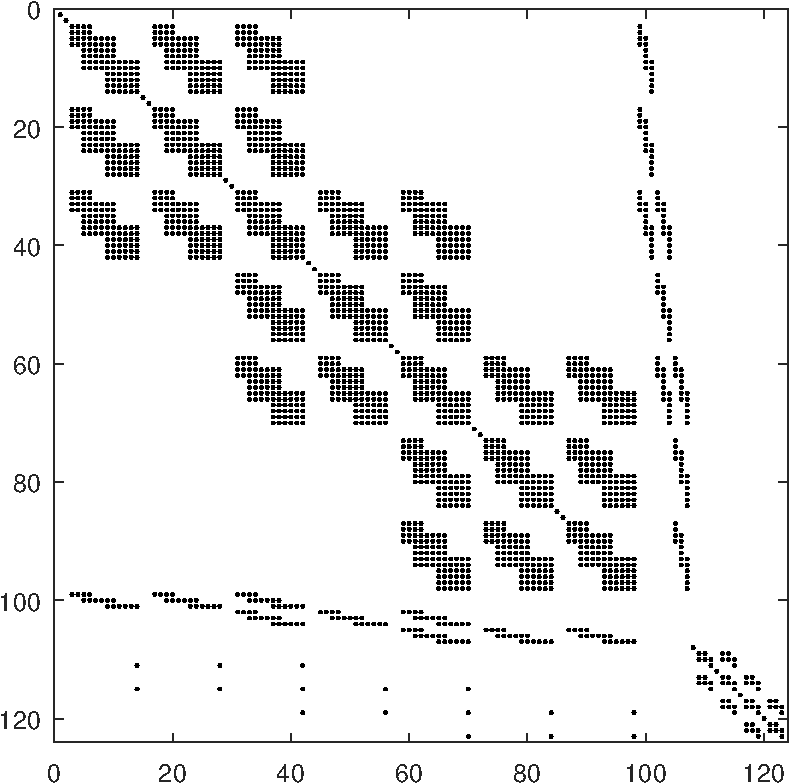
\includegraphics[width=0.6\textwidth]{figs/coarsespy.pdf}
\end{center}
\caption{FIXME block structure of coupled problem}
\label{fig:blockstructure}
\end{figure}


\section{Validation} \label{sec:validation}

FIXME


\section{Discussion and conclusion} \label{sec:discussion}

FIXME among many things cite \cite{LeysingerGudmundsson2004} regarding earlier comparison of stokes to Halfar

FIXME not appreciated that, while for explicit time-stepping schemes the surface mass balance need only be computed at the current ice surface, and at neighboring ice-free locations, in implicit time stepping the surface mass balance must be available to the evolving-geometry model (specifically to the residual-evaluation code) at every location in a 3D neighborhood of the ice surface, and indeed at all 3D locations above the bedrock elevation; a ``potential ice surface mass balance'' is needed at all such locations

\appendix
\section{The shallow ice approximation and its solutions}

The shallow ice approximation (SIA), a widely-used simplified model for the flow of grounded, non-sliding ice \cite{SchoofHewitt2013}, is applied in this paper only for comparison purposes.  It is derived by a small-parameter argument which we recall from Chapter 18 of \cite{Fowler1997}; similar arguments appear in other sources e.g.~\cite{GreveBlatter2009}.

Let $[H]$, $[L]$, $[U]$, and $[\tau]$ denote typical thickness, horizontal extent, horizontal velocity, and vertical-plane shear stress values, respectively, of a glacier.  We consider $\eps = [H]/[L]$ as the small parameter; for a mountain glacier we might have $\eps \approx 0.1$ but for the Greenland ice sheet $\eps \in (10^{-3},10^{-2})$ is reasonable.  We scale the kinematic variables $x,y \sim [L]$, $z \sim [H] = \eps [L]$, $u,v \sim [U]$, and $w \sim \eps [U]$.\footnote{Recall this means, for example, that we introduce new ``hatted'' variables via $x=[L]\hat x$, $y=[L]\hat y$, and $z=[H] \hat z$.  The equations are rewritten in the new variables and then the hats are removed.}  We suppose stress components $\tau_{xz},\tau_{yz}$ scale with $[\tau]$ and $\tau_{xx},\tau_{yy},\tau_{xy}$ with $\eps[\tau]$.   The pressure perturbation from the hydrostatic condition, namely $p-\rhoi g (h - z)$, is scaled with $\eps [\tau]$ also; this means that $p-\rhoi g (h - z)=\eps[\tau]\hat{\delta p}$.  With these scalings, plus certain additional relationships among the scale factors \cite{Fowler1997}, equation \eqref{forcebalance} yields
    $$\frac{\partial\tau_{xz}}{\partial z} + O(\eps^2) = \frac{\partial h}{\partial x}, \qquad \frac{\partial\tau_{yz}}{\partial z} + O(\eps^2) = \frac{\partial h}{\partial y}.$$
The shear strain rates are dominated by the $z$ derivatives of the horizontal velocity, thus
    $$\tau_{xz} = \nu\left(\frac{\partial u}{\partial z} + \eps^2 \frac{\partial w}{\partial z}\right), \qquad \tau_{yz} = \nu\left(\frac{\partial v}{\partial z} + \eps^2 \frac{\partial w}{\partial y}\right).$$
Also, the norm of the deviatoric stress satisfies $|\tau|^2 = \tau_{xz}^2 + \tau_{yz}^2 + O(\eps^2)$ and the stress-free condition at the surface $z=h$ becomes $\tau_{xz} = O(\eps^2)$ and $\tau_{yz} = O(\eps^2)$.  Note that incompressibility \eqref{incompressible} is unaltered by the scaling.

The strong form of the SIA arises from dropping terms of order $O(\eps^2)$ from the scaled equations and returning to the original, unscaled variables.  In order to compactly state these equations let $\bm{\tau}=\left<\tau_{xz},\tau_{yz}\right>$ denote the remaining shear stress components and $\bm{\omega}=\left<\frac{1}{2} \frac{\partial u}{\partial z},\frac{1}{2} \frac{\partial v}{\partial z}\right>$ the corresponding strain rates.  Note that \eqref{viscflowlaw} implies $|\bm{\tau}|=B_n |\bm{\omega}|^{1/n}$, where $|\cdot|$ denotes the ordinary Euclidean norm on $\RR^2$, and thus that $\bm{\omega} = A_n |\bm{\tau}|^{n-1} \bm{\tau}$ where $A_n=(B_n)^{-n}$.  We now have the following equations for the shear stresses and the velocity,
\begin{equation}
\frac{\partial\bm{\tau}}{\partial z} = \rhoi g \grad h, \qquad \Div \bu = 0, \qquad \bm{\omega} = A_n |\bm{\tau}|^{n-1} \bm{\tau}, \label{siavectorized}
\end{equation}
subject to $\bm{\tau}=0$ at the surface $z=h$ and $\bu=0$ on the base $z=b$.

The SIA stress equations \eqref{siavectorized} can be vertically-integrated to give a formulas for the horizontal velocity.  A first integral gives $\bm{\tau} = - \rhoi g (h-z) \grad h$, thus
    $$\left<\frac{\partial u}{\partial z},\frac{\partial v}{\partial z}\right> = - 2 A_n (\rhoi g)^n (h-z)^n |\grad h|^{n-1} \grad h.$$
Integrating again we determine the horizontal velocity at any point within the ice:
\begin{equation}
\left<u,v\right> = - \frac{2 A_n (\rhoi g)^n}{n+1} \left((h-b)^{n+1} - (h-z)^{n+1}\right) |\grad h|^{n-1} \grad h.  \label{siavelocity}
\end{equation}

The result in \eqref{siavelocity} is not actually our model for ice flow, but rather it has three ancillary purposes.  First, in combination with the hydrostatic pressure computation $p=\rhoi g (h-z)$, and vertical integration of the incompressibility equation to approximate $w$, it provides a fast computation of an initial iterate for a nonlinear Stokes solver.  Second, the computation of \eqref{siavelocity} on a given mesh defines our ``work unit'' when evaluating Stokes solver performance on that mesh.  Third, when combined with the surface kinematical equation, \eqref{siavelocity} can be used to derive a nonlinear and degenerate diffusion equation for the ice sheet thickness \cite{Fowler1997}.  We will use the following exact similarity solution of this diffusion equation as a source of synthetic ice sheet initial states in certain numerical experiments.

This solution arises from the $n=3$, flat-bed ($b=0$), and zero surface mass balance ($a=0$) case.  By integrating equation \eqref{siavelocity} vertically one may show that the scaled surface kinematical equation implies that the evolving ice thickness function $H(t,x,y)\ge 0$ solves
\begin{equation}
\frac{\partial H}{\partial t} = \Gamma \Div \left(H^5 |\grad H|^2 \grad H\right). \label{sia}
\end{equation}
on the set where $H>0$ \cite{Fowler1997}, where $\Gamma = \frac{2}{5} A_3 (\rhoi g)^3$.  References \cite{Bueler2016,Calvoetal2002,JouvetBueler2012} consider the rigorous meaning of this free boundary problem.  P.~Halfar \cite{Halfar1981} observed that \eqref{sia} has an exact similarity solution with $\lim_{t\to 0} H$ equal to a Dirac delta function, and that this solution is asymptotically stable.  In 3D \cite{Halfar1983} the solution is a circular dome which spreads radially while thinning, with constant-in-time total volume.  Denoting the radial coordinate as $r=(x^2+y^2)^{1/2}$, the solution is of the form $H(t,r) = t^{-\alpha} \varphi(s)$ with similarity variable $s=t^{-\beta} r$ and $\alpha=1/9$ and $\beta=1/18$.  If a center thickness $H_0$ and radius $R_0$ are given then, on the set where $H$ is positive \cite{Bueleretal2005},
\begin{equation}
H(t,x,y) = H_0 \left(\frac{t}{t_0}\right)^{-\alpha} \left\{1 - \left[\left(\frac{t}{t_0}\right)^{-\beta} \frac{r}{R_0}\right]^{4/3}\right\}^{3/7}. \label{halfar}
\end{equation}
The characteristic time is found by $t_0 = (\beta/\Gamma) (7/4)^3 R_0^4 H_0^{-7}$.  The corresponding 2D Halfar solution $H(t,x)$ \cite{Halfar1981}, in one horizontal dimension, is of the same form as \eqref{halfar} but with $r$ replaced by $x$ and with $\alpha=\beta=1/11$.

\small

\bigskip
\bibliography{simp}
\bibliographystyle{siam}

\end{document}
